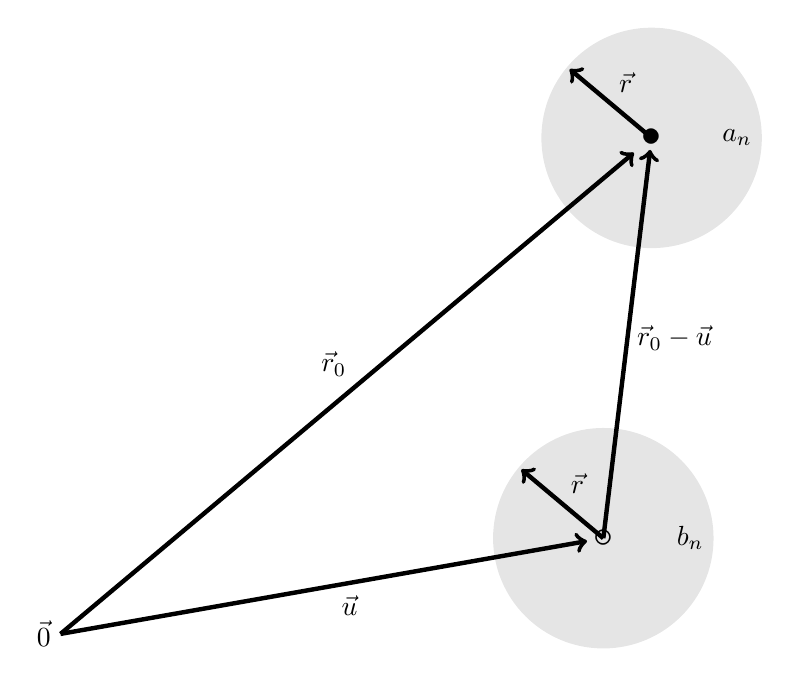
\begin{tikzpicture}[scale=5]
% Parameters
\def\lengthscale{1.4};
\def\radius{0.2*\lengthscale}
\def\arrowStart{0};
\def\arrowScale{0.97};

\pgfmathsetmacro\evalX{cos(140)*\radius}
\pgfmathsetmacro\evalY{sin(140)*\radius}

\pgfmathsetmacro\micX{cos(10)*\lengthscale}
\pgfmathsetmacro\micY{sin(10)*\lengthscale}

\pgfmathsetmacro\listenerX{cos(40)*1.4*\lengthscale}
\pgfmathsetmacro\listenerY{sin(40)*1.4*\lengthscale}

% Arrows
%\draw[ultra thick,->] ({\arrowStart*\evalX},{\arrowStart*\evalY}) -- (\arrowScale*\evalX,\arrowScale*\evalY);
%\node[above right] at (0.5*\evalX,0.5*\evalY){$\vec{r}$};
%\fill [color=black,opacity=0.1] (0,0) circle (\radius);

\draw[ultra thick,->] ({\arrowStart*\evalX+\micX},{\arrowStart*\evalY+\micY}) -- (\arrowScale*\evalX+\micX,\arrowScale*\evalY+\micY);
\node[above right] at (0.5*\evalX+\micX,0.5*\evalY+\micY){$\vec{r}$};
\fill [color=black,opacity=0.1] (\micX,\micY) circle (\radius);

\draw[ultra thick,->] ({\arrowStart*\evalX+\listenerX},{\arrowStart*\evalY+\listenerY}) -- (\arrowScale*\evalX+\listenerX,\arrowScale*\evalY+\listenerY);
\node[above right] at (0.5*\evalX+\listenerX,0.5*\evalY+\listenerY){$\vec{r}$};
\fill [color=black,opacity=0.1] (\listenerX,\listenerY) circle (\radius);

\draw[ultra thick,->] ({\arrowStart*\micX},{\arrowStart*\micY}) -- (\arrowScale*\micX,\arrowScale*\micY);
\node[below right] at (0.5*\micX,0.5*\micY){$\vec{u}$};

\draw[ultra thick,->] ({\arrowStart*\listenerX},{\arrowStart*\listenerY}) -- (\arrowScale*\listenerX,\arrowScale*\listenerY);
\node[above left] at (0.5*\listenerX,0.5*\listenerY){$\vec{r}_0$};

\draw[ultra thick,->] ({(\listenerX-\micX)*\arrowStart+\micX},{(\listenerY-\micY)*\arrowStart+\micY}) -- ({(\listenerX-\micX)*\arrowScale+\micX},{(\listenerY-\micY)*\arrowScale+\micY});
\node[right] at ({(\listenerX-\micX)*0.5+\micX},{(\listenerY-\micY)*0.5+\micY}){$\vec{r}_0 - \vec{u}$};

% Origin
\node[left] at (0,0){$\vec{0}$};

% Mic position
\node at (\micX,\micY){\Large $\circ$};
\node[left] at (\micX+\radius,\micY){$b_n$};

% Listener position
\node at (\listenerX,\listenerY){\Large $\bullet$};
\node[left] at (\listenerX+\radius,\listenerY){$a_n$};
\end{tikzpicture}